\documentclass[a4paper,11pt]{article}

\usepackage[utf8]{inputenc}

\usepackage{minted}
\usepackage{graphicx}

\begin{document}


\title{
    \textbf{Sorting report}
}
\author{Jonathan Karlsson}
\date{Fall 2023}

\maketitle

\section*{Introduction}
This assignment was to create three different sorting algorithms and benchmark them. The algorithms were
selection sort, insertion sort and merge sort. 


\section*{Implementation}
\subsection*{Selection sort}
The selection sort is a simple algorithm which works by going through every element in an array and then going through every 
element from the current index in a second for loop this is done to save the smallest element after the first element. Then the smallest element and
the current element from the first for loop is swapped. This is then done until there are no more elements.
\begin{minted}{java}
for (int i = 0; i < array.length -1; i++) {
    int candidate = i;
    for (int j = i; j < array.length ; j++) {
        if(array[j] < array[candidate])
            candidate = j; 
    }
    int move = array[candidate];
    array[candidate] = array[i];
    array[i] = move;
}
\end{minted}

\subsection*{Insertion sort}
Insertion sort was implemented by once again using a for loop to go through every element. However after that it is different from selection sort,
as insertion sort then uses a second for loop to go from the current element to the start of the array as long as the element before is larger than the 
selected element. Every time it is larger the swap method is called. 
\begin{minted}{java}
for (int i = 0; i < array.length; i++) {
    for (int j = i; j > 0 && array[j-1] > array[j]; j--) {
        swap(array, j, j-1);
    }
}
\end{minted}
The swap method just takes the first argument and swaps it with the second argument, which here is j and j-1.
\begin{minted}{java}
public static void swap(int[] array, int first, int second) {
    int temp = array[first];
    array[first] = array[second];
    array[second] = temp;
}
\end{minted}

\subsection*{Merge sort}
The merge sort is a bit more complicated than insertion or selection sort as it uses recursion instead of for loops.
The sort method starts by generating an aux array and then calling a sort method with the original array, an aux array, lo as 0 and hi as the final element.
\begin{minted}{java}
public void sort(int[] org) {
    if (org.length == 0)
    return;
    int[] aux = new int[org.length];
    sort(org, aux, 0, org.length -1);
    }
\end{minted}
The second sort method works by checking if the highest element is not the lowest. If it is not, it sets mid as the mid point of the array it was given, then
it calls itself with mid as the high point. After that is finishied it calls itself with mid+1 as the low point and finally it merges the two sorted arrays using merge. 
This works with recursion as the arrays will keep shrinking until there is only 1 element left. Then it will get mereged with another element and that continues until the whole 
array is sorted.
\begin{minted}{java}
private static void sort(int[] org, int[] aux, int lo, int hi) {
    if (lo != hi) {
    int mid = (lo + hi)/2;
    sort(org,aux,lo,mid);
    sort(org,aux,mid+1,hi);
    merge(org, aux, lo, mid, hi);
    }
}
\end{minted}
The merge method works by first copying every element from org to aux. Then it sets i, as the lo and j as mid + 1. Then it runs through every element from lo to hi.
Finally a couple of if statements are run to check how the array should be merged so that it gets sorted.
The first if statement cheks if i is greater than mid, if it is set the current element to aux[j] and increase j.
Else if j is greater than hi set the current element to aux[i] and increase i. Else if aux[i] is lower than aux[j] set the current element to aux[i] and increase i.
Finally if non of the other if statements were true set the current elemetn to aux[j] and increase j.
\begin{minted}{java}
private static void merge(int[] org, int[] aux, int lo, int mid, int hi) {
    for(int i = lo; i <= hi;i++) {
        aux[i] = org[i];
    }

    int i = lo;
    int j = mid+1; 

    for ( int k = lo; k <= hi; k++) {
        
        if(i > mid) {
            org[k] = aux[j];
            j++;
        }

        else if(j > hi) {
            org[k] = aux[i];
            i++;
        }

        else if(aux[i] < aux[j]) {
            org[k] = aux[i];
            i++;
        }

        else {
        org[k] = aux[j];
        j++;
        }
    }
}
\end{minted}

\section*{Benchmark}
The benchmark for the three sorting algorithms were written so that a random array of size n was created, then each algorithm was
given a copy of this array to sort 1000 times, then the minimum time was saved. A fourth algorithm, an alternative version of
the merge algorithm were the elements get copied to the aux array before the sort was also benchmarked, this decreased the time the algorithm took for higher values. A table containing some of the 
values can be found below. Full table found at the end of the report.

\begin{table}[h]
    \begin{center}
    \scalebox{0.85}{
    \begin{tabular}{l|c|c|c|c}
    \textbf{n} & \textbf{Selection({\textmu}s)} & \textbf{Insertion({\textmu}s)}& \textbf{Merge({\textmu}s)}& \textbf{Merge(alt)({\textmu}s)}\\
    \hline
    100 &      4 &       2 &      5 &      5 \\
    200 &     14 &       6 &      8 &      8 \\
    300 &     30 &      13 &     13 &     11 \\
    400 &     50 &      24 &     17 &     13 \\
   1000 &    272 &     131 &     53 &     43 \\
   1600 &    657 &     336 &     92 &     78 \\
  25600 & 166623 &  108856 &   1893 &   1713 \\
  51200 & 622164 &  333003 &   3930 &   3587 \\


    \end{tabular}
    }
    \caption{The results of the benchmark for the different sorting algorithms}
    \label{tab:table1}
    \end{center}
\end{table}

\noindent
A graph for the result was also created. This graph shows that both merge sort algorithms follow the same path, and both insertion and seleciton sort follow a similar path. 
The merge sort algorithms seem to follow the $O(nlog(n))$ while the other two algorithms follows $O(n^2)$
\begin{figure}[h]
    \centering    
    
    \scalebox{0.75}{% GNUPLOT: LaTeX picture with Postscript
\begingroup
  \makeatletter
  \providecommand\color[2][]{%
    \GenericError{(gnuplot) \space\space\space\@spaces}{%
      Package color not loaded in conjunction with
      terminal option `colourtext'%
    }{See the gnuplot documentation for explanation.%
    }{Either use 'blacktext' in gnuplot or load the package
      color.sty in LaTeX.}%
    \renewcommand\color[2][]{}%
  }%
  \providecommand\includegraphics[2][]{%
    \GenericError{(gnuplot) \space\space\space\@spaces}{%
      Package graphicx or graphics not loaded%
    }{See the gnuplot documentation for explanation.%
    }{The gnuplot epslatex terminal needs graphicx.sty or graphics.sty.}%
    \renewcommand\includegraphics[2][]{}%
  }%
  \providecommand\rotatebox[2]{#2}%
  \@ifundefined{ifGPcolor}{%
    \newif\ifGPcolor
    \GPcolortrue
  }{}%
  \@ifundefined{ifGPblacktext}{%
    \newif\ifGPblacktext
    \GPblacktextfalse
  }{}%
  % define a \g@addto@macro without @ in the name:
  \let\gplgaddtomacro\g@addto@macro
  % define empty templates for all commands taking text:
  \gdef\gplbacktext{}%
  \gdef\gplfronttext{}%
  \makeatother
  \ifGPblacktext
    % no textcolor at all
    \def\colorrgb#1{}%
    \def\colorgray#1{}%
  \else
    % gray or color?
    \ifGPcolor
      \def\colorrgb#1{\color[rgb]{#1}}%
      \def\colorgray#1{\color[gray]{#1}}%
      \expandafter\def\csname LTw\endcsname{\color{white}}%
      \expandafter\def\csname LTb\endcsname{\color{black}}%
      \expandafter\def\csname LTa\endcsname{\color{black}}%
      \expandafter\def\csname LT0\endcsname{\color[rgb]{1,0,0}}%
      \expandafter\def\csname LT1\endcsname{\color[rgb]{0,1,0}}%
      \expandafter\def\csname LT2\endcsname{\color[rgb]{0,0,1}}%
      \expandafter\def\csname LT3\endcsname{\color[rgb]{1,0,1}}%
      \expandafter\def\csname LT4\endcsname{\color[rgb]{0,1,1}}%
      \expandafter\def\csname LT5\endcsname{\color[rgb]{1,1,0}}%
      \expandafter\def\csname LT6\endcsname{\color[rgb]{0,0,0}}%
      \expandafter\def\csname LT7\endcsname{\color[rgb]{1,0.3,0}}%
      \expandafter\def\csname LT8\endcsname{\color[rgb]{0.5,0.5,0.5}}%
    \else
      % gray
      \def\colorrgb#1{\color{black}}%
      \def\colorgray#1{\color[gray]{#1}}%
      \expandafter\def\csname LTw\endcsname{\color{white}}%
      \expandafter\def\csname LTb\endcsname{\color{black}}%
      \expandafter\def\csname LTa\endcsname{\color{black}}%
      \expandafter\def\csname LT0\endcsname{\color{black}}%
      \expandafter\def\csname LT1\endcsname{\color{black}}%
      \expandafter\def\csname LT2\endcsname{\color{black}}%
      \expandafter\def\csname LT3\endcsname{\color{black}}%
      \expandafter\def\csname LT4\endcsname{\color{black}}%
      \expandafter\def\csname LT5\endcsname{\color{black}}%
      \expandafter\def\csname LT6\endcsname{\color{black}}%
      \expandafter\def\csname LT7\endcsname{\color{black}}%
      \expandafter\def\csname LT8\endcsname{\color{black}}%
    \fi
  \fi
    \setlength{\unitlength}{0.0500bp}%
    \ifx\gptboxheight\undefined%
      \newlength{\gptboxheight}%
      \newlength{\gptboxwidth}%
      \newsavebox{\gptboxtext}%
    \fi%
    \setlength{\fboxrule}{0.5pt}%
    \setlength{\fboxsep}{1pt}%
    \definecolor{tbcol}{rgb}{1,1,1}%
\begin{picture}(7200.00,5040.00)%
    \gplgaddtomacro\gplbacktext{%
      \csname LTb\endcsname%%
      \put(1210,704){\makebox(0,0)[r]{\strut{}$1$}}%
      \put(1210,1527){\makebox(0,0)[r]{\strut{}$100$}}%
      \put(1210,2350){\makebox(0,0)[r]{\strut{}$10000$}}%
      \put(1210,3173){\makebox(0,0)[r]{\strut{}$1\times10^{6}$}}%
      \put(1210,3996){\makebox(0,0)[r]{\strut{}$1\times10^{8}$}}%
      \put(1210,4819){\makebox(0,0)[r]{\strut{}$1\times10^{10}$}}%
      \put(1342,484){\makebox(0,0){\strut{}$100$}}%
      \put(3162,484){\makebox(0,0){\strut{}$1000$}}%
      \put(4983,484){\makebox(0,0){\strut{}$10000$}}%
      \put(6803,484){\makebox(0,0){\strut{}$100000$}}%
    }%
    \gplgaddtomacro\gplfronttext{%
      \csname LTb\endcsname%%
      \put(209,2761){\rotatebox{-270}{\makebox(0,0){\strut{}time in µs}}}%
      \put(4072,154){\makebox(0,0){\strut{}n}}%
      \csname LTb\endcsname%%
      \put(2794,3311){\makebox(0,0)[r]{\strut{}Selection}}%
      \csname LTb\endcsname%%
      \put(2794,3091){\makebox(0,0)[r]{\strut{}Insertion}}%
      \csname LTb\endcsname%%
      \put(2794,2871){\makebox(0,0)[r]{\strut{}Merge}}%
      \csname LTb\endcsname%%
      \put(2794,2651){\makebox(0,0)[r]{\strut{}Merge(alt)}}%
      \csname LTb\endcsname%%
      \put(2794,2431){\makebox(0,0)[r]{\strut{}nlog(n)}}%
      \csname LTb\endcsname%%
      \put(2794,2211){\makebox(0,0)[r]{\strut{}n*n}}%
    }%
    \gplbacktext
    \put(0,0){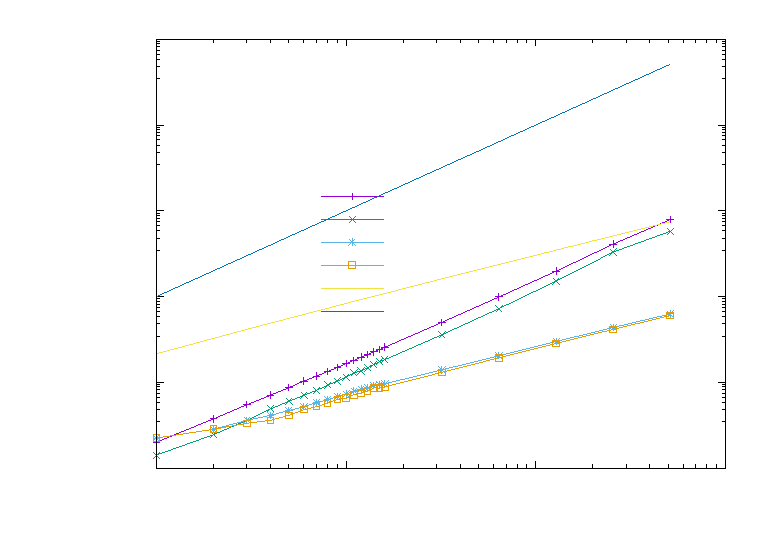
\includegraphics[width={360.00bp},height={252.00bp}]{disp}}%
    \gplfronttext
  \end{picture}%
\endgroup
}
    \caption{Visualization of the different sorting algorithms}   
    \label{tab:figure1} 
    
    \end{figure}
\section*{Conclusion}
It seems that the merge sort algorithm is definitely faster even though it is more complicated and harder to understand. However it could be argued that it is
worse if you have small amount of memory as it requires the use of a second array, instead of only using the original array as the firts two algorithms do.




\newpage
\section*{Full table}
\begin{table}[ht]
    \begin{center}
    \scalebox{0.9}{
    \begin{tabular}{l|c|c|c|c}
    \textbf{n} & \textbf{Selection({\textmu}s)} & \textbf{Insertion({\textmu}s)}& \textbf{Merge({\textmu}s)}& \textbf{Merge(alt)({\textmu}s)}\\
    \hline
    100 &      4 &       2 &      5 &      5 \\
    200 &     14 &       6 &      8 &      8 \\
    300 &     30 &      13 &     13 &     11 \\
    400 &     50 &      24 &     17 &     13 \\
    500 &     75 &      36 &     22 &     17 \\
    600 &    107 &      50 &     27 &     23 \\
    700 &    140 &      65 &     34 &     27 \\
    800 &    179 &      86 &     39 &     33 \\
    900 &    222 &     107 &     47 &     40 \\
   1000 &    272 &     131 &     53 &     43 \\
   1100 &    325 &     166 &     62 &     51 \\
   1200 &    382 &     183 &     69 &     55 \\
   1300 &    442 &     217 &     73 &     63 \\
   1400 &    510 &     258 &     85 &     74 \\
   1500 &    581 &     302 &     87 &     73 \\
   1600 &    657 &     336 &     92 &     78 \\
   3200 &   2497 &    1282 &    195 &    170 \\
   6400 &   9760 &    5216 &    416 &    373 \\
  12800 &  38940 &   22908 &    893 &    801 \\
  25600 & 166623 &  108856 &   1893 &   1713 \\
  51200 & 622164 &  333003 &   3930 &   3587 \\


    \end{tabular}
    }
    \caption{The results of the benchmark for the different sorting algorithms (full table)}
    \label{tab:table2}
    \end{center}
\end{table}

\end{document}
